%%Para utilizar este template siga o tutorial disponível em http://www.biblioteca.ufc.br/wp-content/uploads/2015/09/tutorial-sharelatex.pdf
%%%%%%%%%%%%%%%%%%%%%%%%%%%%%%%%%%%%%%%%%%%%%%%%%%%%%%%
%% Você deve criar uma conta no Overleaf. Depois,    %%
%% vá nas opções no canto esquerdo superior da tela  %%
%% e clique em "Copiar Projeto". Dê um novo nome pa- %%
%% ra o projeto.                                     %%
%%                                                   %%
%% Os principais desenvolvedores deste template são: %%
%%                                                   %%
%%            Ednardo Moreira Rodrigues              %%
%%       (Doutor em Engenharia Elétrica - UFC)       %%
%%(Coord. do Grupo de Astronomia da Seara da Ciência)%%
%%                      &                            %%
%%            Alan Batista de Oliveira               %%
%%           (Engenheiro Eletricista - UFC)          %%
%%                                                   %%
%% Consultoria Bibliotecária                         %%
%%                                                   %%
%%  Versão 2016 - ShareLaTeX:                        %% 
%%                                                   %%
%% - Francisco Edvander Pires Santos;                %%
%% - Juliana Soares Lima;                            %%
%% - Izabel Lima dos Santos;                         %%
%% - Kalline Yasmin Soares Feitosa;                  %%
%% - Eliene Maria Vieira de Moura.                   %%
%% ------------------------------------------------- %% 
%%  Versão 2019,2020 - Overleaf:                     %%
%%                                                   %%
%%  Biblioteca de Ciências Humanas:                  %%
%% - Francisco Edvander Pires Santos;                %%
%% - Juliana Soares Lima;                            %%
%% - Eliene Maria Vieira de Moura;                   %%
%% - Edmundo Moreira de Sousa Filho.                 %%
%%                                                   %%
%% Biblioteca da FEAAC:                              %%
%% - Izabel Lima dos Santos;                         %%
%% - Kalline Yasmin Soares Feitosa;                  %%
%% - Kleber Lima dos Santos.                         %%
%%                                                   %%
%%  Biblioteca do Curso de Física:                   %%
%% - Aline Rodrigues de Lima Mendes;                 %%
%% - Maria de Jesus Silva dos Santos.                %%
%%                                                   %%
%%  Biblioteca Central do Campus do Pici:            %%
%% - Raquel da Silva Nascimento.                     %%
%% - Felipe Ferreira da Silva                        %%
%%  Versão 2019,2020 - Overleaf:                     %%
%%  ------------------------------------------------ %%
%%  Versão de 2022 - Overleaf                        %%
%%                                                   %%
%%   a) Felipe Ferreira da Silva                        %%
%%   b) Ednardo Moreira Rodrigues                       %%
%%   c) Comissão de Normalização do Sistema de          %%
%%      Bibliotecas da UFC                              %%
%%                                                   %%
%% Colaboradores                                     %%
%%                                                   %%
%% -Andrei Bosco Bezerra Torres                      %% 
%% (Professor - Sistemas e Mídias Digitais -         %%
%% Instituto Universidade Virtual - UFC)             %%
%% Tiago Alves Lima                                  %% 
%% (Aluno de Mestrado em Eng. Elétrica)              %%
%%                                                   %%
%% Grande parte do trabalho foi adaptado do template %%
%% da UECE elaborado por:                            %%
%% Thiago Nascimento  (UECE)                         %%
%% Project available on:                             %%
%% https://github.com/thiagodnf/uecetex2             %%
%%                                                   %%
%% "Dúvidas, esclarecimentos ou sugestões podem ser  %%
%% enviadas para o seguinte e-mail:                  %%
%%                                                   %%
%%             bu@ufc.br               %%
%%                                                   %%
%% As últimas atualizações estão descritas no inicio %%
%% do arquivo "README.md".                           %%
%%                                                   %%
%%%%%%%%%%%%%%%%%%%%%%%%%%%%%%%%%%%%%%%%%%%%%%%%%%%%%%%

\documentclass[        
    a4paper,          % Tamanho da folha A4
    12pt,             % Tamanho da fonte 12pt
    chapter=TITLE,    % Todos os capitulos devem ter caixa alta
    section=Title,    % Todas as secoes devem ter caixa alta somente na primeira letra
    subsection=Title, % Todas as subsecoes devem ter caixa alta somente na primeira letra
    oneside,          % Usada para impressao em apenas uma face do papel
    english,          % Hifenizacoes em ingles
    spanish,          % Hifenizacoes em espanhol
    brazil,           % Ultimo idioma eh o idioma padrao do documento
    fleqn             % Comente esta linha se quiser centralizar as equacoes. Comente também a linha 65 abaixo
]{abntex2}

% Para utilizar este template siga o tutorial disponível em http://www.biblioteca.ufc.br/wp-content/uploads/2015/09/tutorial-sharelatex.pdf

%%%%%%%%%%%%%%%%%%%%%%%%%%%%%%%%%%%%%%%%%%%%%%%%%%%%%%%
%% Você deve criar uma conta no Overleaf. Depois,    %%
%% vá nas opções no canto esquerdo superior da tela  %%
%% e clique em "Copiar Projeto". Dê um novo nome pa- %%
%% ra o projeto.                                     %%
%%                                                   %%
%% Os principais desenvolvedores deste template são: %%
%%                                                   %%
%%            Ednardo Moreira Rodrigues              %%
%%       (Doutor em Engenharia Elétrica - UFC)       %%
%%(Coord. do Grupo de Astronomia da Seara da Ciência)%%
%%                      &                            %%
%%            Alan Batista de Oliveira               %%
%%           (Engenheiro Eletricista - UFC)          %%
%%                                                   %%
%% Consultoria Bibliotecária                         %%
%%                                                   %%
%%  Versão 2016 - ShareLaTeX:                        %% 
%%                                                   %%
%% - Francisco Edvander Pires Santos;                %%
%% - Juliana Soares Lima;                            %%
%% - Izabel Lima dos Santos;                         %%
%% - Kalline Yasmin Soares Feitosa;                  %%
%% - Eliene Maria Vieira de Moura.                   %%
%%                                                   %% 
%%  Versão 2019 - Overleaf:                          %%
%%                                                   %%
%%  Biblioteca de Ciências Humanas:                  %%
%% - Francisco Edvander Pires Santos;                %%
%% - Juliana Soares Lima;                            %%
%% - Eliene Maria Vieira de Moura;                   %%
%% - Edmundo Moreira de Sousa Filho.                 %%
%%                                                   %%
%% Biblioteca da FEAAC:                              %%
%% - Izabel Lima dos Santos;                         %%
%% - Kalline Yasmin Soares Feitosa;                  %%
%% - Kleber Lima dos Santos.                         %%
%%                                                   %%
%%  Biblioteca do Curso de Física:                   %%
%% - Aline Rodrigues de Lima Mendes;                 %%
%% - Maria de Jesus Silva dos Santos.                %%
%%                                                   %%
%%  Biblioteca Central do Campus do Pici:            %%
%% - Raquel da Silva Nascimento.                     %%
%% - Felipe Ferreira da Silva                        %%
%%                                                   %%
%% Colaboradores                                     %%
%%                                                   %%
%% -Andrei Bosco Bezerra Torres                      %% 
%% (Professor - Sistemas e Mídias Digitais -         %%
%% Instituto Universidade Virtual - UFC)             %%
%% Tiago Alves Lima                                  %% 
%% (Aluno de Mestrado em Eng. Elétrica)              %%
%%                                                   %%
%% Grande parte do trabalho foi adaptado do template %%
%% da UECE elaborado por:                            %%
%% Thiago Nascimento  (UECE)                         %%
%% Project available on:                             %%
%% https://github.com/thiagodnf/uecetex2             %%
%%                                                   %%
%% "Dúvidas, esclarecimentos ou sugestões podem ser  %%
%% enviadas para o seguinte e-mail:                  %%
%%                                                   %%
%%             atendimentobch@ufc.br                 %%
%%                                                   %%
%% As últimas atualizações estão descritas no inicio %%
%% do arquivo "README.md".                           %%
%%                                                   %%
%%%%%%%%%%%%%%%%%%%%%%%%%%%%%%%%%%%%%%%%%%%%%%%%%%%%%%%

% Importações de pacotes
\usepackage[utf8]{inputenc}                         % Acentuação direta
\usepackage[T1]{fontenc}                            % Codificação da fonte em 8 bits
\usepackage{graphicx}                               % Inserir figuras
\usepackage{amsfonts, amssymb, amsmath}             % Fonte e símbolos matemáticos
\usepackage{booktabs}                               % Comandos para tabelas
\usepackage{verbatim}                               % Texto é interpretado como escrito no documento
\usepackage{multirow, array}                        % Múltiplas linhas e colunas em tabelas
\usepackage{indentfirst}                            % Endenta o primeiro parágrafo de cada seção.
\usepackage{listings}                               % Utilizar codigo fonte no documento
\usepackage{xcolor}
\usepackage{microtype}                              % Para melhorias de justificação?
\usepackage[portuguese,ruled,lined]{algorithm2e}    % Escrever algoritmos
\usepackage{algorithmic}                            % Criar Algoritmos  
%\usepackage{float}                                 % Utilizado para criação de floats
\usepackage{amsgen}
\usepackage{lipsum}                                 % Usar a simulação de texto Lorem Ipsum
%\usepackage{titlesec}                              % Permite alterar os títulos do documento
% \usepackage{tocloft}                                % Permite alterar a formatação do Sumário
\usepackage{tocloft}

\usepackage{etoolbox}                               % Usado para alterar a fonte da Section no Sumário
\usepackage[nogroupskip,nonumberlist]{glossaries}   % Permite fazer o glossario. A apcao "sort=use" faz com que as siglas aparecam na lista conformse sao usadas no texto.

\usepackage[format=plain,justification=justified,skip=0pt,singlelinecheck = false,labelsep=colon]{caption}            % Altera o comportamento da tag caption. Algumas opcoes do caption so podem ser alternada no arquivo "antex2.cls, linhas 334 a 348.

\usepackage[alf, abnt-emphasize=bf, recuo=0cm, abnt-etal-cite=2, abnt-etal-list=0, abnt-etal-text=it]{lib/ufcTexcite}  % Citações padrão UFC/ABNT NBR 6023 de 2018
%\usepackage[bottom]{footmisc}                      % Mantém as notas de rodapé sempre na mesma posição
%\usepackage{times}                                 % Usa a fonte Times
%%%%%%%%%%%%%%%%%%% AVISO %%%%%%%%%%%%%%%%%%%%%%%%%%%%%%%%%%%%%%%%
%descomente as duas linhas abaixo para alterar o texto de Times New Roman para Arial:

%\usepackage{helvet}
%\renewcommand{\familydefault}{\sfdefault}  % Usa a fonte Arial              
%%%%%%%%%%%%%%%%%%%%%%%%%%%%%%%%%%%%%%%%%%%%%%%%%%%%%%%%%%%%%%%%%%

\usepackage{mathptmx}         % Usa a fonte Times New Roman			%\usepackage{lmodern}         % Usa a fonte Latin Modern
%\usepackage{subfig}          % Posicionamento de figuras
%\usepackage{scalefnt}        % Permite redimensionar tamanho da fonte
%\usepackage{color, colortbl} % Comandos de cores
%\usepackage{lscape}          % Permite páginas em modo "paisagem"
%\usepackage{ae, aecompl}     % Fontes de alta qualidade
%\usepackage{picinpar}        % Dispor imagens em parágrafos
%\usepackage{latexsym}        % Símbolos matemáticos
%\usepackage{upgreek}         % Fonte letras gregas
\usepackage{appendix}         % Gerar o apendice no final do documento
\usepackage{paracol}          % Criar paragrafos sem identacao
\usepackage{lib/ufcTexcite}
\usepackage{lib/ufcTex}	      % Biblioteca com as normas da UFC para trabalhos academicos
\usepackage{pdfpages}         % Incluir pdf no documento
\usepackage{amsmath}          % Usar equacoes matematicas
%\usepackage[opções]{subfigure} %plotar subfiguras


\makeglossaries % Organiza e gera a lista de abreviaturas, simbolos e glossario
\makeindex      % Gera o Indice do documento         

\renewcommand{\labelitemi}{\textendash} %Altera os marcadores de itemize para 

% \color{teal}




\setlength{\mathindent}{0pt} %Complementa o alinhamento de equações para totalmente a esquerda.

%%%%%%%%%%%%%%%%%%%%%%%%%%%%%%%%%%%%%%%%%%%%%%%%%%%%%
%%                     ATENCAO                     %%
%%%%%%%%%%%%%%%%%%%%%%%%%%%%%%%%%%%%%%%%%%%%%%%%%%%%%
%  Qual e o nivel do trabalho academico que voce esta 
% escrevendo? Retire o simbolo "%" apenas de um dos 
% quatro topicos abaixo refente ao nível do seu traba
% -lho.

%\trabalhoacademico{tccgraduacao}
%\trabalhoacademico{tccespecializacao}
\trabalhoacademico{dissertacao}
%\trabalhoacademico{tese}

%%%%%%%%%%%%%%%%%%%%%%%%%%%%%%%%%%%%%%%%%%%%%%%%%%%%%

% Define se o trabalho e uma qualificacao
% Coloque 'nao' para versao final do trabalho

\ehqualificacao{nao}

% Remove as bordas vermelhas e verdes do PDF gerado
% Coloque 'sim' pare remover

\removerbordasdohyperlink{sim} 

% Adiciona a cor Azul a todos os hyperlinks

\cordohyperlink{nao}

%%%%%%%%%%%%%%%%%%%%%%%%%%%%%%%%%%%%%%%%%%%%%%%%%%%%%
%%         Informacao sobre a instituicao          %%
%%%%%%%%%%%%%%%%%%%%%%%%%%%%%%%%%%%%%%%%%%%%%%%%%%%%%

\ies{Universidade Federal do Ceará}
\iessigla{UFC}
\centro{Centro de Tecnologia}
\departamento{Departamento de Engenharia Elétrica}

%%%%%%%%%%%%%%%%%%%%%%%%%%%%%%%%%%%%%%%%%%%%%%%%%%%%%
%%        Informacao para TCC de Graduacao         %%
%%%%%%%%%%%%%%%%%%%%%%%%%%%%%%%%%%%%%%%%%%%%%%%%%%%%%

\graduacaoem{Engenharia Xxxxxxx}
\habilitacao{bacharel} % Ou licenciado(a)

% AVISO: Caso necessario alterar o texto de apresenta-
% cao da Especializacao, ir a pasta "lib", arquivo 
% "ufctex.sty" na linha 502.


%%%%%%%%%%%%%%%%%%%%%%%%%%%%%%%%%%%%%%%%%%%%%%%%%%%%%
%%     Informacao para TCC de Especializacao       %%
%%%%%%%%%%%%%%%%%%%%%%%%%%%%%%%%%%%%%%%%%%%%%%%%%%%%%

\especializacaoem{Yyyyyyyyy}

% AVISO: Caso necessario alterar o texto de apresenta-
% cao da Especializacao, ir a pasta "lib", arquivo 
% "ufctex.sty" na linha 507.

%%%%%%%%%%%%%%%%%%%%%%%%%%%%%%%%%%%%%%%%%%%%%%%%%%%%%
%%         Informacao para Dissertacao             %%
%%%%%%%%%%%%%%%%%%%%%%%%%%%%%%%%%%%%%%%%%%%%%%%%%%%%%

\programamestrado{Programa de Pós-Graduação em Engenharia Elétrica}
\nomedomestrado{Mestrado Acadêmico em Engenharia Elétrica}
\mestreem{Engenharia Elétrica}
\areadeconcentracaomestrado{Engenharia Elétrica}

% AVISO: Caso necessario alterar o texto de apresenta-
% cao da dissertacao, ir a pasta "lib", arquivo 
% "ufctex.sty" na linha 511.

%%%%%%%%%%%%%%%%%%%%%%%%%%%%%%%%%%%%%%%%%%%%%%%%%%%%%
%%               Informação para Tese              %%
%%%%%%%%%%%%%%%%%%%%%%%%%%%%%%%%%%%%%%%%%%%%%%%%%%%%%

\programadoutorado{Programa de Pós-Graduação em Xxxxxx}
\nomedodoutorado{Doutorado em Xxxxxxx}
\doutorem{Engenharia Xxxxxx}
\areadeconcentracaodoutorado{Engenharia Xxxxxxx}

% AVISO: Caso necessario alterar o texto de apresenta-
% cao da tese, ir a pasta "lib", arquivo "ufctex.sty" 
% na linha 515.

%%%%%%%%%%%%%%%%%%%%%%%%%%%%%%%%%%%%%%%%%%%%%%%%%%%%%
%%      Informacoes relacionadas ao trabalho       %%
%%%%%%%%%%%%%%%%%%%%%%%%%%%%%%%%%%%%%%%%%%%%%%%%%%%%%

\autor{Davi Alexandre Paiva}
\titulo{}
\data{2023}
\local{Fortaleza}

% Exemplo: \dataaprovacao{01 de Janeiro de 2012}
\dataaprovacao{}

%%%%%%%%%%%%%%%%%%%%%%%%%%%%%%%%%%%%%%%%%%%%%%%%%%%%%
%%           Informação sobre o Orientador         %%
%%%%%%%%%%%%%%%%%%%%%%%%%%%%%%%%%%%%%%%%%%%%%%%%%%%%%

\orientador{Prof. Dr. Wilkley Bezerra Correia}
\orientadories{Universidade Federal do Ceará (UFC)}
\orientadorcentro{Centro de Tecnologia (CT)}
\orientadorfeminino{nao} % Coloque 'sim' se for do sexo feminino

%%%%%%%%%%%%%%%%%%%%%%%%%%%%%%%%%%%%%%%%%%%%%%%%%%%%%
%%          Informação sobre o Coorientador        %%
%%%%%%%%%%%%%%%%%%%%%%%%%%%%%%%%%%%%%%%%%%%%%%%%%%%%%

% Deixe o nome do coorientador em branco para remover do documento

\coorientador{}
\coorientadories{Universidade Coorientador (SIGLA)}
\coorientadorcentro{Centro do Coorientador (SIGLA)}
\coorientadorfeminino{nao} % Coloque 'sim' se for do sexo feminino

%%%%%%%%%%%%%%%%%%%%%%%%%%%%%%%%%%%%%%%%%%%%%%%%%%%%%
%%              Informação sobre a banca           %%
%%%%%%%%%%%%%%%%%%%%%%%%%%%%%%%%%%%%%%%%%%%%%%%%%%%%%

% Atenção! Deixe em branco o nome do membro da banca para remover da folha de aprovacao

% Exemplo de uso:
% \membrodabancadois{Prof. Dr. Fulano de Tal}
% \membrodabancadoisies{Universidade Federal do Ceará - UFC}


\membrodabancadois{}
\membrodabancadoiscentro{}
\membrodabancadoisies{}
\membrodabancatres{}
\membrodabancatrescentro{}
\membrodabancatresies{}
% \membrodabancaquatro{Prof. Dr. Xxxxxxx Xxxxxx Xxxxxxx}
% \membrodabancaquatrocentro{Centro de Ciências e Tecnologia (CCT)}
% \membrodabancaquatroies{Universidade do Membro da Banca cinco (SIGLA)}
% \membrodabancacinco{Prof. Dr. Xxxxxxx Xxxxxx Xxxxxxx}
% \membrodabancacincocentro{Teste}
% \membrodabancacincoies{Universidade do Membro da Banca seis (SIGLA)}
% \membrodabancaseis{Prof. Dr. Xxxxxxx Xxxxxx Xxxxxxx}
% \membrodabancaseiscentro{}
% \membrodabancaseisies{Universidade do Membro da Banca sete (SIGLA)}


\begin{document}

% Elementos pré-textuais
\imprimircapa
\imprimirfolhaderosto{}
% \imprimirfichacatalografica{1-pre-textuais/ficha-catalografica}
%\imprimirerrata{elementos-pre-textuais/errata}
\imprimirfolhadeaprovacao
% \imprimirdedicatoria{1-pre-textuais/dedicatoria}
% \imprimiragradecimentos{1-pre-textuais/agradecimentos}
% \imprimirepigrafe{1-pre-textuais/epigrafe}
\imprimirresumo{1-pre-textuais/resumo}
% \imprimirabstract{1-pre-textuais/abstract}
\renewcommand*\listfigurename{Lista de Figuras} 
% Se você comentar esta linha o título da lista fica: LISTA DE ILUSTRAÇÕES
% \imprimirlistadeilustracoes
% \imprimirlistadetabelas
% \imprimirlistadequadros
% \imprimirlistadealgoritmos
% \imprimirlistadecodigosfonte
% \imprimirlistadeabreviaturasesiglas
% \imprimirlistadesimbolos{1-pre-textuais/lista-de-simbolos}   
\imprimirsumario

\setcounter{table}{0} % Deixe este comando antes da primeira tabela.

% Elementos textuais
\textual
\chapter{Introdução}
\label{cap:introducao}

%Para começar a usar este \textit{template}, na plataforma \textit{ShareLatex}, vá nas opções (três barras vermelhas horizontais) no canto esquerdo superior da tela e clique em "Copiar Projeto" e dê um novo nome para o projeto. 



%Testando o símbolo $\symE$

%\lipsum[5]  % Simulador de texto, ou seja, é um gerador de lero-lero.

%	\begin{alineas}
%		\item Lorem ipsum dolor sit amet, consectetur adipiscing elit. Nunc dictum sed tortor nec viverra.
%		\item Praesent vitae nulla varius, pulvinar quam at, dapibus nisi. Aenean in commodo tellus. Mauris molestie est sed justo malesuada, quis feugiat tellus venenatis.
%		\item Praesent quis erat eleifend, lacinia turpis in, tristique tellus. Nunc dictum sed tortor nec viverra.
%		\item Mauris facilisis odio eu ornare tempor. Nunc dictum sed tortor nec viverra.
%		\item Curabitur convallis odio at eros consequat pretium.
%	\end{alineas}



Um sistema industrial é composto por sensores, atuadores, sinalizadores, controladores entre outros componentes voltados para a realização de determinada cadeia de processos dentro de uma linha de produção. Tal que para realizar determinado processo é necessário uma sincronia entre diversos equipamentos, sensores e atuadores ao longo da planta industrial. Além do desafio de sincronizar uma gama de processos, os sistemas modernos possuem a necessidade de adaptar-se a novas variações e configurações, abrindo espaço para máquinas e sistemas com programação mais robusta e reconfigurável. 
Dado este desafio, as redes de Petri coloridas se oferecem como uma ótima ferramenta de modelagem para os sistemas modernos de manufatura em linha de produção em que há um aumento da versatilidade e flexibilidade da estrutura e também a necessidade de uma programação com alto nível de abstração. 
\cite{WENZELBURGER2019492}

De acordo com
%\cite{discrete}
, as redes de Petri têm sido consideradas com um modelo adequado para um controle supervisório com o objetivo de abranger uma grande classe de problemas e explorar a análise algébrica necessária para otimização. Tratando-se também da análise para a planta não alcançar determinadas marcações indesejadas;

As redes de Petri também são uma ferramenta de modelagem inicial para o algoritmo de programação com ferramentas intrínsecas que analisam o algoritmo para evitar que o sistema entre em exceções,
%\cite{embeddedOO}

% An industrial system is composed of sensors, actuators, signals, controllers and other components dedicated to the implementation of a certain process in a production line. So that to achieve a certain process, there is a need for synchronization between different equipment throughout the plant.

A planta industrial escolhida para este trabalho é relacionada a um processo de montagem, que é composto por um sistema de três agentes, que são duas esteiras e um robô. Uma esteira recebe a parte superior da peça (tampa) e a segunda recebe a parte inferior da peça (base), para posicionar as peças em um local determinado da esteira tem-se o prendedor, uma estrutura metálica que prende a peça à borda da esteira, tal prendedor possui dois tipos de movimento, o de prender e de soltar a peça. Para movimentar a tampa e montá-la em cima da base utiliza-se  o terceiro agente, um braço robótico cartesiano, que possui um movimento no eixo X, ortogonal às esteiras e um movimento no eixo Z, que sobe e desce para levantar e baixar a peça da tampa, respectivamente, através de um atuador pneumático que prende a peça à ponta do braço robótico. O algoritmo de sincronia dos agentes e componentes do processo, tais como atuadores, manipuladores, esteiras e sensores foi modelado por redes de Petri coloridas.

%The industrial plant chosen for this work is related to an assembly process, where it has two conveyors, one that receives the upper part of the object (lid) and the second receives the lower part of the object (base), to position the parts in a determined location of the conveyor there is the clamp, a metal structure that holds the part to the edge of the conveyor, such clamp has two types of movement, to hold and to release the parts. To move the lid and mount it on top of the base, a Cartesian robotic arm is used, which moves on the X axis, orthogonal to the conveyors, and moves on the Z axis, which goes up and down to raise and lower the lid part respectively. .

Para modelagem e controle desse sistema composto por vários agentes, escolheu-se a abordagem por redes de Petri coloridas. As redes de Petri  coloridas são uma ferramenta gráfica e matemática que se adaptam bem a um grande numero de aplicações, tais como protocolos de comunicação, controle de oficinas de fabricação. 
A complexidade dos sistemas, em particular o de fabricação automatizada, leva a uma decomposição de vários níveis de controle, tais como planejamento, escalonamento, coordenação global, coordenação de sub-sistemas e controle direto (autômatos programáveis conectados aos sensores e aos atuadores). %\cite{vallete}
% For modeling and control of this system composed of several agents, the Petri net approach was chosen. The Petri net is a graphical and mathematical tool that adapts well to a large number of applications, such as communication protocols, control of manufacturing workshops. The complexity of systems, particularly automated manufacturing, leads to a decomposition of several levels of control, such as planning, scheduling, global coordination, subsystem coordination and direct control (programmable automata connected to sensors and actuators).

Posteriormente à modelagem por redes de Petri, tal rede será programada utilizando linguagem de programação de auto nível através do paradigma de orientação a objeto, facilitando assim a implementação em sistemas reais, comunicação em auto nível entre o sistema e outros elementos da industria, como clps, supervisórios, sistemas web e possibilitando maior flexibilidade na programação, manutenção e simplificação do código além das ferramentas de análise do modelo a partir da análise da rede de Petri correspondente.

Um sistema multiagente é um sistema que possui mais de um agente, representado por uma entidade independente das outras entidades. Tais entidades se comunicam para a sincronia e execução de um determinado objetivo. No sistema de montagem de peça, considera-se uma entidade como um mecanismo robótico, e outras duas entidades como as esteiras industrias, de modo que o robô é uma entidade independente, que não possui o controle e funcionamento dependente das outras entidades. Assim como o robô as esteiras também têm o funcionamento e controle independente entre si. Para alcançar o objetivo comum de montar as peças os agentes se comunicam entre si através de um protocolo que permite informar o estado de cada agente.

Para a modelagem do sistema em redes de Petri são utilizados os lugares, transições e fichas. O lugar pode ser interpretado como uma condição, um estado associado, por exemplo, sensor ligado, eixo em movimento, peça na posição, etc. Já a transição é associada a uma evento que ocorre no sistema, a um acionamento proposto, tal como movimentar a peça, movimentar robô, acionar a esteira, entre outros. Por fim as fichas são uma indicação que a condição associada ao lugar é satisfeita.

Em 
%\cite{design}, 
sistemas de manufatura reorganizáveis são modelados pela linguagem UML, para descrever as reconfigurações do sistema e na segunda fase  os diagramas são transformados em submodelos da rede de Petri e a relação entre os submodelos e subsistemas são sintetizados em um modelo de rede de Petri de auto nível. Os dois métodos podem analisar comportamentos importantes em relação as propriedades do sistema que são vitais para a modelagem prática dos mesmos.

Em 
%\cite{hybridOO} 
é feita a modelagem de um sistema de produção híbrida, baseada em redes de Petri representando as partes discretas do sistema, equações diferencias representando as partes contínuas e paradigma de orientação a objetos para lidar com a complexidade se sistemas reais, em que cada sub rede é relacionada a uma classe modelando o comportamento de cada objeto da classe. Na dinâmica do sistema a marcação representa o presente estado do objeto. Cada grupo de ação é representada por uma classe eque possui um modelo definido pela RP. 

No presente artigo, para a associação entre os elementos básicos de uma rede de Petri (lugar, transição, fichas) e os elementos básicos de uma planta industrial (sensores, atuadores), modelou-se as seguintes associações, todos os sensores e atuadores da planta são representados por lugares na rede de Petri, tal que o mesmo possui uma ou nenhuma ficha representando respectivamente o estado de ligado ou desligado), acionado ou não acionado, e as transições são lógicas de comando que relacionam lugares e memórias no sistema. 


% De outra forma, abordagens mais simplificadas e de fácil ...

% Em se tratando de soluções numéricas ...

% Um grande desafio presente ...

\begin{comment}   

\section{Objetivos}
\subsection{Objetivos gerais}
% O presente trabalho dedica-se ....


\subsection{Objetivos específicos}
% Os objetivos específicos deste trabalho podem ser resumidos em
\begin{itemize}
    \item Modelagem ... ;
    \item Abordagem ...;
    \item Implementação ....; 
\end{itemize}

\end{comment}

\begin{comment}   
\section{Justificativa}
% Uma vez que ....
\end{comment}

\begin{comment}   
 \section{Motivação}
A abordagem .... 
\end{comment}

\begin{comment}   
\section{Produção científica}
Ao longo do desenvolvimento desta dissertação, foram publicados ou submetidos a
congressos ou periódicos os seguintes artigos:
\begin{itemize}
    \item PAIVA, Davi Alexandre et al. A simple procedure for modeling and identification of a test bench 4-DOF manipulator. In: Congresso Brasileiro de Automática-CBA. 2020.
\end{itemize}
\end{comment}

\section{Organização do trabalho}
Para a estruturação do presente trabalho, adota-se a seguinte metodologia de estudo

\begin{enumerate}
\item 
\textbf{Introdução:} Este capítulo contém as premissas básicas de estudo e evolução dos temas recorrentes na área de Controle Multiagentes. Ainda incluem-se os princípios básicos de apresentação do projeto, tais como os objetivos, a justificativa e a motivação do estudo.

\item \textbf{Sistema Multiagentes: } Partindo-se do princípio mais básico relacionado a modelagem de sistemas multiagentes. Assim, definem-se as representações matemáticas e gráficas de um sistema multiagente assim como técnicas de controle Cooperativo. Por fim são repassadas as principais técnicas de modelagem, representação em grafos e controle de sistemas multiagentes. 
    
\item \textbf{Redes de Petri: } 
    
\item \textbf{Simulação:} 
    
\item \textbf{Conclusão:} Por fim, este último capítulo trata das considerações gerais sobre os conceitos apresentados e uma discussão crítica acerca dos resultados de simulação.

\end{enumerate}

	

\chapter{Sistema Multiagentes}

\section{Teoria dos Grafos}
No estudo da interação e comportamento entre sistemas dinâmicos, as interconexões entre os agentes e o fluxo de informações formam uma rede de comunicação. Essa rede é modelada através da teoria dos grafos em que cada sistema é representado por um nó, também chamado de agente.
% Adicionar Referência do livro que fala sobre

Um grafo é um par $G = (V, E)$, tal que $V = \{v_{1},v_{2}, ...,v_{N}\}$ é um conjunto de $N$ nós ou vértices e $E$ um conjunto de vetores ou arcos. Um elemento pertencente a $E$ é um par $(v_{i}, v_{j})$ tal que é um vetor que liga $v_{i}$ à $v_{j}$, e é representado como uma flecha em que a cauda está em $v_{i}$ e a ponta em $v_{j}$ como demonstrado na figura ~\ref{fig:nos_arestas_grafos}. 
% Adicionar Grafo exemplo desenhado : exemplo de nós e arcos em um grafo

\begin{figure}[hb]
    \centering
    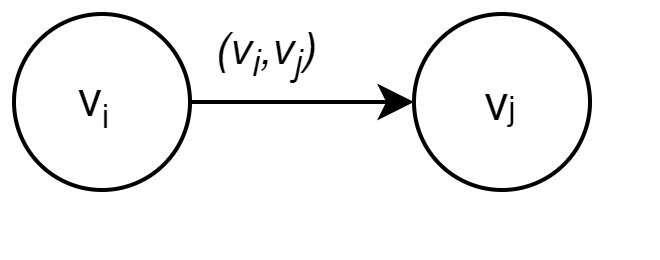
\includegraphics[scale=0.3]{figures/Multiagente/ex_grafo2.png}
    \caption{Exemplo de nós e arestas em um grafo}
    \label{fig:nos_arestas_grafos}
\end{figure}

Os graus de liberdade de entrada de um dado nó $v_i$ é definido como o número de vetores que a ponta da flecha se encontra em $v_i$. Do mesmo modo, os graus de liberdade de saída de um nó $v_i$ é dado pelo número de vetores que em $v_i$ se encontra a cauda da flecha.

Associado à cada aresta de um elemento em $E = (v_i, v_j)$ tem-se um peso $a_{ij} > 0$. O peso $a_{ij}$ representa a força de interação entre os nós $v_i$ e $v_j$. De modo que quanto maior o peso maior a influência tem o comportamento do agente $j$ sobre o agente $i$.
    %revisar esse parágrafo
Um grafo é dito bidirecional se e somente se $a_{ij} \neq 0$ e $a_{ji} \neq 0$, então tem-se que a comunicação entre agentes flui bidirecionalmente. Um grafo é dito unidirecional se $a_{ij} = a_{ji}$, para qualquer $i$ e $j$.


\section{Teoria algébrica dos grafos e consenso do controle cooperativo}

O controle cooperativo estuda a dinâmica de sistemas dinâmicos com múltiplos agentes com iterações um com o outro através de uma comunicação em grafo. 
O grafo representa as iterações e comunicações entre agentes. O objetivo do controle cooperativo é garantir a sincronia entre o comportamento e estados dos agentes, de modo que para cada agente só é disponível que as informações sejam entre o agente com os agentes vizinhos.

\subsection{Representação matricial dos grafos}
A estrutura e propriedade dos grafos podem ser estudadas examinando as propriedades de certas matrizes associadas. Dados os pesos $a{_ij}$ associados, o grafo pode ser representado pela \textbf{Matriz de Adjacência} ou conectividade $A = [a_{ij}]$, com $a_{ij}>0$ $se$ $(v_{j},v_{i}) \in E $ e $a_{ij}$ caso contrário.   
Define-se duas propriedades locais dos grafos, o graus de entrada e os graus de saída.
Os graus de entrada de um nó $v_{i}$ é definido pela equação \ref{eq:InDegree}, tal que $d_{i}$ é o somatório dos pesos $a_{ij}$ da linha $i$-th.

\begin{equation} \label{eq:InDegree}
    d_{i} = \displaystyle\sum_{j=1}^{N}a_{ij}
\end{equation}

Os graus de saída de um nó $v_{i}$ é definido pela equação \ref{eq:OutDegree}, tal que $d_{i}$ é o somatório dos pesos $a_{ij}$ da coluna $i$-th.

\begin{equation}\label{eq:OutDegree}
    d_{i}^0 = \displaystyle\sum_{j = 1}^{N}a_{ji}
\end{equation}

Define-se duas propriedades globais dos grafos, o diâmetro do grafo , dada pela maior distância entre dois nós e o volume de entrada $(in)-volume$, dado pela soma dos nós de entrada
\begin{equation}
    VolG=\displaystyle\sum_{i}d_{i}
\end{equation}

\subsection{Matriz de Grafo Laplaciana}
Uma definição importante aplicada a sistemas multiagentes é a \textbf{Matriz Laplaciana}, que auxilia o estudo das propriedades da dinâmica do grafo de multiagentes. A mesma é obtida através da operação entre duas matrize, a Matriz Diagonal e a Matriz de Adjacência.
Define-se a matriz diagonal de graus de entrada, pela equação \ref{eq:matrizDiagonal}, em que para um agente $i$, tem-se o elemento $d_{i}$ como o somatório das flechas que apontam para o dado agente.
\begin{equation}\label{eq:matrizDiagonal}
    D = diag\{d_{i}\}
\end{equation}
Por fim a matriz Laplaciana $L$ é definida como $L = D-A$, tal que $D$ é a matriz Diagonal e $A$ é a matriz de Adjacência.
\\
Um exemplo de matriz laplaciana associada ao grafo pode ser ilustrada através da figura \ref{fig:exemplo_grafo}, em que a matriz Diagonal $D$ é dada pela matriz \ref{eq:matriz_d1}. 

\begin{figure}
    \centering
    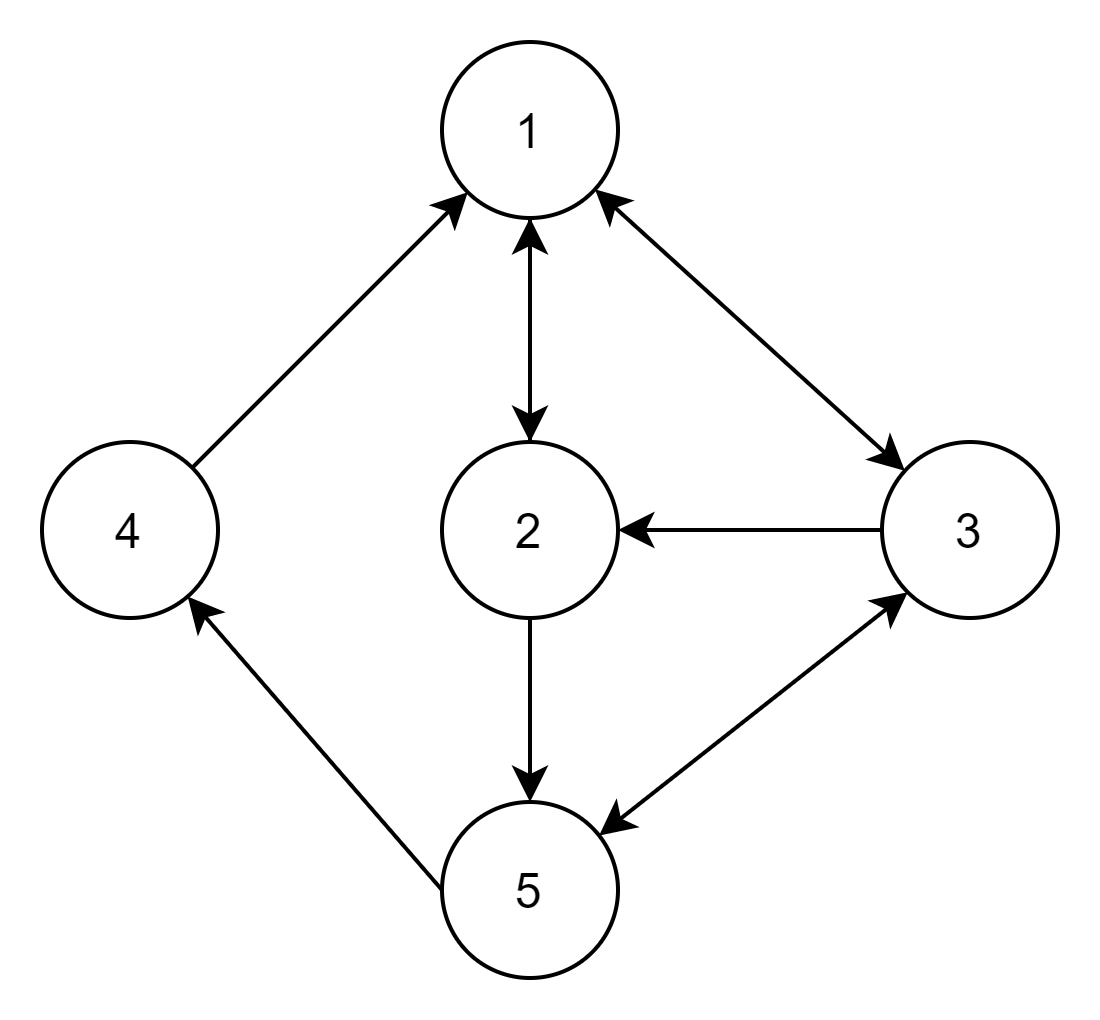
\includegraphics[scale=0.2]{figures/Multiagente/ex_grafos1.png}
    \caption{Exemplo de um grafo}
    \label{fig:exemplo_grafo}
\end{figure}

\begin{equation}\label{eq:matriz_d1}
    D = \begin{bmatrix}
         3 & 0 & 0 & 0 & 0 \\ % graus de entrada do agente 1
         0 & 2 & 0 & 0 & 0 \\ % graus de entrada do agente 2
         0 & 0 & 2 & 0 & 0 \\ % graus de entrada do agente 3
         0 & 0 & 0 & 1 & 0 \\ % graus de entrada do agente 4
         0 & 0 & 0 & 0 & 2 \\ % graus de entrada do agente 5
    \end{bmatrix}
\end{equation}

A matriz A, dada pela Matriz de Adjacência \ref{eq:matriz_A1}.
\begin{equation}\label{eq:matriz_A1}
    A = \begin{bmatrix}
         0 & 1 & 1 & 0 & 0 \\ % conectividade do agente 1  
         1 & 0 & 0 & 0 & 1 \\ % conectividade do agente 2
         1 & 1 & 0 & 0 & 1 \\ % conectividade do agente 3 
         1 & 0 & 0 & 0 & 0 \\ % conectividade do agente 4 
         0 & 0 & 1 & 1 & 0 \\ % conectividade do agente 5 
    \end{bmatrix}
\end{equation}
Por fim, a matriz Laplaciana é dada por $L = D - A$.
\begin{equation}\label{eq:matriz_L1}
    L = \begin{bmatrix}
         3 & -1 & -1 & 0 & 0 \\ 
         -1 & 2 & 0 & 0 & -1 \\ 
         -1 & -1 & 2 & 0 & -1 \\ 
         -1 & 0 & 0 & 1 & 0 \\ 
         0 & 0 & -1 & -1 & 2 \\ 
    \end{bmatrix}
    = \begin{bmatrix}
         3 & 0 & 0 & 0 & 0 \\ % graus de entrada do agente 1
         0 & 2 & 0 & 0 & 0 \\ % graus de entrada do agente 2 
         0 & 0 & 2 & 0 & 0 \\ % graus de entrada do agente 3
         0 & 0 & 0 & 1 & 0 \\ % graus de entrada do agente 4
         0 & 0 & 0 & 0 & 2 \\ % graus de entrada do agente 5
    \end{bmatrix}
    - \begin{bmatrix}
         0 & 1 & 1 & 0 & 0 \\ % conectividade do agente 1  
         1 & 0 & 0 & 0 & 1 \\ % conectividade do agente 2
         1 & 1 & 0 & 0 & 1 \\ % conectividade do agente 3 
         1 & 0 & 0 & 0 & 0 \\ % conectividade do agente 4 
         0 & 0 & 1 & 1 & 0 \\ % conectividade do agente 5 
    \end{bmatrix}
\end{equation}


\section{Consenso com Integrador único}
Para o estudo inicial de controle cooperativo, tem-se a análise de um sistema multiagente formado por agentes $i$ com dinâmica dada por um integrador escalar único, modelada pela equação \ref{eq:int_Unico}
\begin{equation}\label{eq:int_Unico}
    \dot x_{i}  = u_{i} 
\end{equation}
com $x_{i}, u_{i} \in R $ . Isso corresponde que cada nó do grafo $G$, possui um agente com memória.

\subsubsection{Protocolo de controle distribuído para o consenso}
Para cada agente $i$, considere o protocolo de controle local dado pela equação \ref{eq:protocolo_controle_local}
\begin{equation}\label{eq:protocolo_controle_local}
    u_{i} = \sum\limits_{j \in N_{i}} a_{ij} (x_{j} - x_{i})
\end{equation}
com $a_{ij}$ sendo o peso de interação entre os estados dos agentes.Essa equação é conhecida como protocolo de votação local, em que o estado de cada agente depende tão somente do estado do agente vizinho, e a entrada de controle depende da da diferença dos estados em relação aos agentes vizinhos. De modo que percebe-se que se todos os estados forem os mesmo a entrada de controle tende a zero $\dot x_{i} = u_{i} = 0$.

Para a dinâmica de integrador único, é desejável que a equação \ref{eq:int_Unico}, resolva o problema de consenso, da dinâmica de malha fechada dada pela equação \ref{eq:consenso_Int_Unico}
\begin{equation}\label{eq:consenso_Int_Unico}
    \dot x_{i} = \sum\limits_{j \in N_{i}} a_{ij} (x_{j} - x_{i})
\end{equation}

Reorganizando a equação \ref{eq:consenso_Int_Unico}, tem-se que a equação. \ref{eq:consenso_Int_Unico_Expandido}
\begin{equation}\label{eq:consenso_Int_Unico_Expandido}
    \dot x_{i} = -x_{i}\sum\limits_{j \in N_{i}} a_{ij} + 
    \sum\limits_{j \in N_{i}} a_{ij}x_{j} = -d_{i}x_{i} + 
   \left[
   \begin{array}{ccc}
   a_{i1}&\cdots&a_{iN} 
    \end{array}
    \right] 
   \left[
   \begin{array}{ccc}
        x_{1} \\
        \vdots \\
        x_{N}
    \end{array}
    \right]
\end{equation}
tal que $d_{i}$ são os graus de liberdade, $x = [x_{1} \cdots x_{N}]$ $\in R^N$ o vetor de estados. Define-se a matriz $D$ como matriz diagonal formada por $D = diag \{d_{i}\}$, organiza-se a 
dinâmica global, através da matriz dada pela equação Laplaciana.
\begin{equation}\label{eq:construcao_laplaciana}
    \begin{aligned}
        \dot x = -Dx +Ax = -(D-A)x \\
        \dot x = u = -Lx 
    \end{aligned}
\end{equation}
Através da equação \ref{eq:construcao_laplaciana}, e da matriz laplaciana de grafo tem-se que a dinâmica de malha fechada pode ser analisada através da matriz laplaciana dada.
Para a dinâmica de integrador único tem-se que se e somente se o grafo possui a topologia de spanning tree, então todos os estados dos nós vão a um valor de consenso dado por $x_{i} = x_{j} = c$. O valor de consenso é dado pela equação \ref{eq:valor_de_consenso}.
\begin{equation}\label{eq:valor_de_consenso}
    \begin{aligned}
        c = \sum\limits_{i = 1}^{N} p_{i}x_{i}(0)
    \end{aligned}
\end{equation}
tal que $w_{1} = [p_{1} \cdots p_{N}]^{T}$, é o vetor normalizado pela esquerda da matriz laplaciana $L$, para $  \lambda_{1} = 0$. De modo que a constante de tempo é dada por \ref{eq:const_tempo} e $\lambda_{2}$ sendo o segundo autovalor da matriz L.
\begin{equation}\label{eq:const_tempo}
   \tau = 1 / \lambda_{2}
\end{equation}


\subsection{Consenso com líder}
Um "(directed) tree" é um um grafo onde todo nó exceto um é chamado de líder, e possui grau de entrada unitário. De modo que todos os outros nós possuem um consenso liderado pelas condições iniciais do líder.
O valor de consenso é dado pela equação \ref{eq:valor_de_consenso}, de modo que $p_{i}$ é o $i-{th}$ componente para o autovetor pela esquerda de $w_{i}$ para $\lambda_{1} = 0$, tal consenso é na verdade a média ponderada das condições iniciais das raízes dos nós ou do líder em um grafo. 
%% Adicionar simulação parecida com a simulação da pág 42 do livro, sobre consenso com líder.
\\
\\
\subsection{Consenso para nós com estados como vetores}
Nas condições de integrador úninco e integrado duplo apresentadas anteriormente os estados são tidos como escalares, para os exemplos em que os estados são vetores tais como $x_{i}, u_{i} \in R^{N}$ tem-se que os vetores globais de estados e controle são respectivamente $x = [x_{1}^{T} \cdots x_{N}^{T}]^{T} \in R^{nN} , 
u = [u_{1}^{T}  \cdots u_{N}^{T}]^{T} \in R^{nN} $ e os elementos dados pelos pesos de consenso $a_{ij}$ e a diagonal $d_{i}$ são multiplicados pela matriz identidade $I_{n}$, de modo que a dinâmica global do sistema é dada pela equação \ref{eq:consenso_vetorial}

\begin{equation}\label{eq:consenso_vetorial}
 \begin{aligned}
    u = -(L \otimes I_{N})x \\
    \dot x = -(L \otimes I_{N}) x
    \end{aligned}
\end{equation}
dado que $\otimes$ é definido como produto de kronecker.

\subsection{Movimento invariante para consenso de primeira ordem}
Para o protocolo de primeira ordem local dado por \ref{eq:construcao_laplaciana} foi garantido que para a topologia de $spannig tree$ o consenso é alcançado. 



\input{2-textuais/3-Redes-de-Petri}
\input{2-textuais/4-Simulacao}
\chapter{Conclusão}

O método de modelagem e controle proposto foi realizado no problema de uma planta industrial envolvendo a sincronia e formação de um grupo de autômatos ao longo de trajetórias pré definidas, em que a partir de alguns eventos modelados pela rede de Petri foi alterado a formação do grupo de autômatos assim como os pontos de sincronia.
O método se apresentou como uma técnica viável e eficiente, pois para aplicações de sistemas com muitos agentes o controle por consenso se apresenta como uma implementação simples sem grande uso de recurso matemático que fornece a sincronia necessária para aplicação de formação ordenada do grupo de autômatos.
No ponto de vista de robustez e adaptabilidade do sistema, observou-se que cada agente respeita as limitações dos agentes vizinhos, seja ela de posição de velocidade, evitando assim colisões e independente da mudança da dinâmica de um agente todo o sistema tem sua dinâmica adaptada, trazendo assim uma sincronia entre os diferentes agentes com diferentes dinâmicas ao longo do sistema.
A principal contribuição desse trabalho é a técnica conjunta de modelagem e controle que  diminui o processamento local em cada agente deixando assim as lógicas de processamento centralizada em um sistema supervisório modelado via rede de petri, além de uma lógica de controle de baixo custo computacional, todavia é necessário uma ótima comunicação entre os agentes,pois a base do controle é dada pela sincronia entre os estados do agente vizinho.
	

% Elementos pós-textuais	
\bibliography{3-pos-textuais/referencias}
% \imprimirglossario %	
% \imprimirapendices
% Adicione aqui os apêndices do seu trabalho
% % \apendice{EXEMPLO DE APÊNDICE}
% \label{ap:A}


% % \apendice{ Questionário utilizado para}
% \label{ap:B}

% \begin{questao}
% 	\item Esta é a primeira questão com alguns itens:
% 		\begin{enumerate}
% 			\item Este é o primeiro item
% 			\item Segundo item
% 		\end{enumerate}
% 	\item Esta é a segunda questão:
% 		\begin{enumerate}
% 			\item Este é o primeiro item
% 			\item Segundo item
% 		\end{enumerate}
% 	\item Lorem ipsum dolor sit amet, consectetur adipiscing elit. Nunc dictum sed tortor nec viverra. consectetur adipiscing elit. Nunc dictum sed tortor nec viverra.
% 		\begin{enumerate}
% 			\item consectetur
% 			\item adipiscing
% 			\item Nunc
% 			\item dictum
% 		\end{enumerate}
% \end{questao}

% % \apendice{ Códigos-fontes utilizados para}
% \label{ap:C}

% \lstinputlisting[language=C++,caption={Hello World em C++}]{figuras/main.cpp}


% \begin{lstlisting}[language=Java,caption={Hello World em Java}]
% public class HelloWorld {
% 	public static void main(String[] args) {
% 		System.out.println("Hello World!");
% 	}
% }
% \end{lstlisting}


% \imprimiranexos
% Adicione aqui os anexos do seu trabalho
% % \anexo{ Exemplo de um anexo}
% \label{an:ex_anexo_a}

% \textcolor{red}{Colocar como anexo o passo a passo de integração do matlab com o coppelia.}




% % \anexo{ Exemplo de um anexo em PDF}
% \label{an:ex_anexo_b}

% O autor pode anexar um \gls{PDF}, traduzido como formato portátil de documento. Veja o código fonte utilizado para anexar o arquivo ``Sikasil.pdf'' que foi colocado dentro da pasta ``anexos'' que por sua vez está dentro da pasta ``elementos-pos-textuais''. Tenha muita atenção na hora de especificar o local do arquivo. Recomenda-se não utilizar caracteres especiais para nomear pastas e, principalmente, arquivos. 

% Pode-se fazer uma descrição sucinta do arquivo anexado.

%Comando para incluir um arquivo em PDF:
% \includepdf[pages={-}]{3-pos-textuais/anexos/Sikasil.pdf}

		
% \imprimirindice

\end{document}